\chapter{Annexes}

\newgeometry{left=0.5cm, right=0.5cm}
\begin{longtable}{| p{12.5cm}| c | c| }
        \textbf{Nom de l'échantillon} & \textbf{Classe réelle} & \textbf{Classe prédite} \\
        \hline
        mémoire et bio.\char`_Audoux Marguerite\char`_Marie-Claire\char`_sample\char`_1.txt & mémoire et bio. & nouvelle \\
        \hline
        mémoire et bio.\char`_Audoux Marguerite\char`_Marie-Claire\char`_sample\char`_3.txt & mémoire et bio. & nouvelle \\
        \hline
        mémoire et bio.\char`_Barbara Charles\char`_L'assassinat du pont rouge\char`_sample\char`_1.txt & mémoire et bio. & roman \\
        \hline
        mémoire et bio.\char`_Bazin René\char`_La Sarcelle Bleue\char`_sample\char`_1.txt & mémoire et bio. & nouvelle \\
        \hline
        mémoire et bio.\char`_Bazin René\char`_La Sarcelle Bleue\char`_sample\char`_3.txt & mémoire et bio. & nouvelle \\
        \hline
        mémoire et bio.\char`_Belot Adolphe\char`_Alphonsine\char`_sample\char`_2.txt & mémoire et bio. & roman \\
        \hline
        mémoire et bio.\char`_Belot Adolphe\char`_Alphonsine\char`_sample\char`_3.txt & mémoire et bio. & roman \\
        \hline
        mémoire et bio.\char`_Boylesve René\char`_Le carrosse aux deux lézards verts\char`_sample\char`_1.txt & mémoire et bio. & nouvelle \\
        \hline
        mémoire et bio.\char`_Boylesve René\char`_Le carrosse aux deux lézards verts\char`_sample\char`_2.txt & mémoire et bio. & roman \\
        \hline
        mémoire et bio.\char`_Daudet Alphonse\char`_Souvenirs d'un homme de lettres\char`_sample\char`_1.txt & mémoire et bio. & nouvelle \\
        \hline
        mémoire et bio.\char`_Daudet Alphonse\char`_Wood'stown\char`_sample\char`_1.txt & mémoire et bio. & nouvelle \\
        \hline
        mémoire et bio.\char`_Dubut de Laforest Jean-Louis\char`_Morphine\char`_sample\char`_2.txt & mémoire et bio. & nouvelle \\
        \hline
        mémoire et bio.\char`_Dubut de Laforest Jean-Louis\char`_Morphine\char`_sample\char`_3.txt & mémoire et bio. & nouvelle \\
        \hline
        mémoire et bio.\char`_Dumas (père) Alexandre\char`_La boule de neige\char`_sample\char`_3.txt & mémoire et bio. & nouvelle \\
        \hline
        mémoire et bio.\char`_Dumas (père) Alexandre\char`_La boule de neige\char`_sample\char`_4.txt & mémoire et bio. & roman \\
        \hline
        mémoire et bio.\char`_Dumas (père) Alexandre\char`_Une aventure d'amour\char`_sample\char`_2.txt & mémoire et bio. & roman \\
        \hline
        mémoire et bio.\char`_Durand Alice dite Gréville Henry\char`_Croquis\char`_sample\char`_3.txt & mémoire et bio. & nouvelle \\
        \hline
        mémoire et bio.\char`_Durand Alice dite Gréville Henry\char`_Croquis\char`_sample\char`_4.txt & mémoire et bio. & nouvelle \\
        \hline
        mémoire et bio.\char`_Eekhoud Georges\char`_La faneuse d'amour\char`_sample\char`_1.txt & mémoire et bio. & nouvelle \\
        \hline
        mémoire et bio.\char`_Eekhoud Georges\char`_La faneuse d'amour\char`_sample\char`_3.txt & mémoire et bio. & nouvelle \\
        \hline
        mémoire et bio.\char`_Eekhoud Georges\char`_La faneuse d'amour\char`_sample\char`_4.txt & mémoire et bio. & nouvelle \\
        \hline
        mémoire et bio.\char`_Feuillet Octave\char`_La petite comtesse\char`_sample\char`_1.txt & mémoire et bio. & roman \\
        \hline
        mémoire et bio.\char`_Féval Paul (père)\char`_La Ville-Vampire (ou bien le malheur d’écrire des romans noirs)\char`_sample\char`_2.txt & mémoire et bio. & nouvelle \\
        \hline
        mémoire et bio.\char`_Féval Paul (père)\char`_La Ville-Vampire (ou bien le malheur d’écrire des romans noirs)\char`_sample\char`_4.txt & mémoire et bio. & roman \\
        \hline
        mémoire et bio.\char`_Féval (père) Paul\char`_La fabrique de crimes\char`_sample\char`_1.txt & mémoire et bio. & roman \\
        \hline
        mémoire et bio.\char`_Galopin Arnould\char`_La ténébreuse affaire de Green-Park\char`_sample\char`_2.txt & mémoire et bio. & nouvelle \\
        \hline
        mémoire et bio.\char`_Galopin Arnould\char`_La ténébreuse affaire de Green-Park\char`_sample\char`_3.txt & mémoire et bio. & nouvelle \\
        \hline
        mémoire et bio.\char`_Gay Sophie\char`_Anatole, Vol. 2\char`_sample\char`_2.txt & mémoire et bio. & roman \\
        \hline
        mémoire et bio.\char`_Gérald-Montméril (pseud. Gérald Mabel et Mme Mairel d'Eslon)\char`_Chryséis au désert\char`_sample\char`_1.txt & mémoire et bio. & nouvelle \\
        \hline
        mémoire et bio.\char`_Gérald-Montméril (pseud. Gérald Mabel et Mme Mairel d'Eslon)\char`_Chryséis au désert\char`_sample\char`_3.txt & mémoire et bio. & nouvelle \\
        \hline
        mémoire et bio.\char`_Gérald-Montméril (pseud. Gérald Mabel et Mme Mairel d'Eslon)\char`_Chryséis au désert\char`_sample\char`_4.txt & mémoire et bio. & roman \\
        \hline
        mémoire et bio.\char`_Ginouvier J.-F.-T.\char`_Gustave et Aspaïs, ou Les victimes des préjugés de l'époque . Par T. Ginouvier - Tome 2 (1826)\char`_sample\char`_3.txt & mémoire et bio. & pamphlet \\
        \hline
        mémoire et bio.\char`_Hémon Louis\char`_Écrits sur le Québec\char`_sample\char`_2.txt & mémoire et bio. & pamphlet \\
        \hline
        mémoire et bio.\char`_Inconnu\char`_Indiscrétions d'une Parisienne. Mademoiselle Figaro (1880)\char`_sample\char`_1.txt & mémoire et bio. & nouvelle \\
        \hline
        mémoire et bio.\char`_Inconnu\char`_Indiscrétions d'une Parisienne. Mademoiselle Figaro (1880)\char`_sample\char`_2.txt & mémoire et bio. & roman \\
        \hline
        mémoire et bio.\char`_Inconnu\char`_Indiscrétions d'une Parisienne. Mademoiselle Figaro (1880)\char`_sample\char`_3.txt & mémoire et bio. & roman \\
        \hline
        mémoire et bio.\char`_Lermina Jules\char`_La deux fois morte\char`_sample\char`_1.txt & mémoire et bio. & nouvelle \\
        \hline
        mémoire et bio.\char`_Lermina Jules\char`_L'énigme\char`_sample\char`_1.txt & mémoire et bio. & nouvelle \\
        \hline
        mémoire et bio.\char`_Loti Pierre\char`_Figures et choses qui passaient\char`_sample\char`_3.txt & mémoire et bio. & nouvelle \\
        \hline
        mémoire et bio.\char`_Loti Pierre\char`_Matelot\char`_sample\char`_1.txt & mémoire et bio. & nouvelle \\
        \hline
        mémoire et bio.\char`_Loti Pierre\char`_Matelot\char`_sample\char`_3.txt & mémoire et bio. & nouvelle \\
        \hline
        mémoire et bio.\char`_Maupassant Guy de\char`_Au soleil\char`_sample\char`_2.txt & mémoire et bio. & nouvelle \\
        \hline
        mémoire et bio.\char`_Maupassant Guy de\char`_Au soleil\char`_sample\char`_3.txt & mémoire et bio. & nouvelle \\
        \hline
        mémoire et bio.\char`_Mazier du Heaume Hippolyte\char`_Voyage d'un jeune grec à Paris. Volume 2\char`_sample\char`_1.txt & mémoire et bio. & pamphlet \\
        \hline
        mémoire et bio.\char`_Méténier Oscar\char`_Le gorille. Roman parisien\char`_sample\char`_1.txt & mémoire et bio. & roman \\
        \hline
        mémoire et bio.\char`_Méténier Oscar\char`_Le gorille. Roman parisien\char`_sample\char`_2.txt & mémoire et bio. & nouvelle \\
        \hline
        mémoire et bio.\char`_Méténier Oscar\char`_Le gorille. Roman parisien\char`_sample\char`_3.txt & mémoire et bio. & roman \\
        \hline
        mémoire et bio.\char`_Musset Paul de\char`_La Chèvre Jaune\char`_sample\char`_1.txt & mémoire et bio. & nouvelle \\
        \hline
        mémoire et bio.\char`_Musset Paul de\char`_La Chèvre Jaune\char`_sample\char`_2.txt & mémoire et bio. & nouvelle \\
        \hline
        mémoire et bio.\char`_Nadaud Marcel\char`_Chignole (la guerre aérienne)\char`_sample\char`_1.txt & mémoire et bio. & nouvelle \\
        \hline
        mémoire et bio.\char`_Nervo Robert de (Baron)\char`_Les Mémoires de mon coupé (1881)\char`_sample\char`_2.txt & mémoire et bio. & nouvelle \\
        \hline
        mémoire et bio.\char`_Nizan Paul\char`_Aden Arabie\char`_sample\char`_1.txt & mémoire et bio. & pamphlet \\
        \hline
        mémoire et bio.\char`_Nizan Paul\char`_Aden Arabie\char`_sample\char`_2.txt & mémoire et bio. & pamphlet \\
        \hline
        mémoire et bio.\char`_Nizan Paul\char`_Aden Arabie\char`_sample\char`_3.txt & mémoire et bio. & pamphlet \\
        \hline
        mémoire et bio.\char`_Ohnet Georges\char`_L'Ame de Pierre\char`_sample\char`_1.txt & mémoire et bio. & nouvelle \\
        \hline
        mémoire et bio.\char`_Ohnet Georges\char`_L'Ame de Pierre\char`_sample\char`_2.txt & mémoire et bio. & nouvelle \\
        \hline
        mémoire et bio.\char`_Ohnet Georges\char`_L'Ame de Pierre\char`_sample\char`_3.txt & mémoire et bio. & roman \\
        \hline
        mémoire et bio.\char`_Pollet Louis Léonard dit Corday Michel\char`_Les révélées\char`_sample\char`_1.txt & mémoire et bio. & nouvelle \\
        \hline
        mémoire et bio.\char`_Pollet Louis Léonard dit Corday Michel\char`_Les révélées\char`_sample\char`_2.txt & mémoire et bio. & nouvelle \\
        \hline
        mémoire et bio.\char`_Ponson du Terrail Pierre\char`_Le Chambrion\char`_sample\char`_1.txt & mémoire et bio. & roman \\
        \hline
        mémoire et bio.\char`_Renard Jules\char`_Poil de carotte\char`_sample\char`_2.txt & mémoire et bio. & nouvelle \\
        \hline
        mémoire et bio.\char`_Rodenbach Georges\char`_Bruges-la-Morte\char`_sample\char`_1.txt & mémoire et bio. & nouvelle \\
        \hline
        mémoire et bio.\char`_Rosny aîné J-H\char`_La Femme disparue\char`_sample\char`_2.txt & mémoire et bio. & roman \\
        \hline
        mémoire et bio.\char`_Sales Pierre\char`_Le sergent Renaud. Aventures parisiennes\char`_sample\char`_1.txt & mémoire et bio. & roman \\
        \hline
        mémoire et bio.\char`_Sand George\char`_Promenades autour d’un village\char`_sample\char`_2.txt & mémoire et bio. & pamphlet \\
        \hline
        mémoire et bio.\char`_Sand George\char`_Promenades autour d’un village\char`_sample\char`_3.txt & mémoire et bio. & pamphlet \\
        \hline
        mémoire et bio.\char`_Sand George\char`_Promenades autour d’un village\char`_sample\char`_4.txt & mémoire et bio. & pamphlet \\
        \hline
        mémoire et bio.\char`_Signol Alphonse\char`_Le Chiffonnier, par Alphonse Signol et Stanislas Macaire - Tome 3 (1831)\char`_sample\char`_2.txt & mémoire et bio. & roman \\
        \hline
        mémoire et bio.\char`_Signol Alphonse\char`_Le Chiffonnier, par Alphonse Signol et Stanislas Macaire - Tome 4 (1831)\char`_sample\char`_1.txt & mémoire et bio. & roman \\
        \hline
        mémoire et bio.\char`_Tardieu Charles Henri\char`_Lettres de Bayreuth\char`_sample\char`_2.txt & mémoire et bio. & pamphlet \\
        \hline
        mémoire et bio.\char`_Toudouze Gustave\char`_La sirène: souvenir de Capri\char`_sample\char`_1.txt & mémoire et bio. & nouvelle \\
        \hline
        mémoire et bio.\char`_Toulet Paul Jean\char`_La jeune fille verte, roman\char`_sample\char`_3.txt & mémoire et bio. & nouvelle \\
        \hline
        mémoire et bio.\char`_Verlaine Paul\char`_Les mémoires d’un veuf\char`_sample\char`_2.txt & mémoire et bio. & pamphlet \\
        \hline
        mémoire et bio.\char`_Verlaine Paul\char`_Mes hôpitaux\char`_sample\char`_1.txt & mémoire et bio. & pamphlet \\
        \hline
        mémoire et bio.\char`_Verlaine Paul\char`_Mes prisons\char`_sample\char`_1.txt & mémoire et bio. & pamphlet \\
        \hline
        mémoire et bio.\char`_Zaccone Pierre\char`_Éric le mendiant\char`_sample\char`_2.txt & mémoire et bio. & nouvelle \\
        \hline
        mémoire et bio.\char`_Zaccone Pierre\char`_La Dame d'Auteuil\char`_sample\char`_3.txt & mémoire et bio. & roman \\
        \hline
        nouvelle\char`_Allary Camille\char`_Au pays des cigales\char`_sample\char`_2.txt & nouvelle & mémoire et bio. \\
        \hline
        nouvelle\char`_Arène Paul\char`_Contes de Provence\char`_sample\char`_2.txt & nouvelle & mémoire et bio. \\
        \hline
        nouvelle\char`_Balzac Honoré de\char`_El Verdugo\char`_sample\char`_1.txt & nouvelle & roman \\
        \hline
        nouvelle\char`_Balzac Honoré de\char`_Esquisse d’un homme d’affaires d’après nature\char`_sample\char`_1.txt & nouvelle & roman \\
        \hline
        nouvelle\char`_Balzac Honoré de\char`_Gambara\char`_sample\char`_2.txt & nouvelle & roman \\
        \hline
        nouvelle\char`_Balzac Honoré de\char`_Le Bal de Sceaux\char`_sample\char`_1.txt & nouvelle & roman \\
        \hline
        nouvelle\char`_Balzac Honoré de\char`_Le Bal de Sceaux\char`_sample\char`_2.txt & nouvelle & roman \\
        \hline
        nouvelle\char`_Balzac Honoré de\char`_Les Secrets de la princesse de Cadignan\char`_sample\char`_1.txt & nouvelle & roman \\
        \hline
        nouvelle\char`_Balzac Honoré de\char`_Maître Cornélius\char`_sample\char`_1.txt & nouvelle & roman \\
        \hline
        nouvelle\char`_Balzac Honoré de\char`_Une passion dans le désert\char`_sample\char`_1.txt & nouvelle & roman \\
        \hline
        nouvelle\char`_Balzac Honoré de\char`_Z. Marcas\char`_sample\char`_1.txt & nouvelle & roman \\
        \hline
        nouvelle\char`_Bellaud E. de\char`_Ces pauvres filles !\char`_sample\char`_1.txt & nouvelle & roman \\
        \hline
        nouvelle\char`_Bellaud E. de\char`_Ces pauvres filles !\char`_sample\char`_3.txt & nouvelle & roman \\
        \hline
        nouvelle\char`_Boissières Ernest\char`_Un crime inconnu\char`_sample\char`_3.txt & nouvelle & mémoire et bio. \\
        \hline
        nouvelle\char`_Bréhat Alfred de\char`_Le bal de l'Opéra\char`_sample\char`_4.txt & nouvelle & mémoire et bio. \\
        \hline
        nouvelle\char`_Bréhat Alfred de\char`_L'hôtel du dragon ; Souvenirs de voyages\char`_sample\char`_1.txt & nouvelle & mémoire et bio. \\
        \hline
        nouvelle\char`_Bréhat Alfred de\char`_L'hôtel du dragon ; Souvenirs de voyages\char`_sample\char`_3.txt & nouvelle & mémoire et bio. \\
        \hline
        nouvelle\char`_Cim Albert\char`_Contes et souvenirs de mon pays\char`_sample\char`_2.txt & nouvelle & mémoire et bio. \\
        \hline
        nouvelle\char`_Claretie Jules\char`_Bouddha\char`_sample\char`_1.txt & nouvelle & mémoire et bio. \\
        \hline
        nouvelle\char`_Colette\char`_Les Vrilles de la vigne\char`_sample\char`_2.txt & nouvelle & mémoire et bio. \\
        \hline
        nouvelle\char`_Crevel René\char`_Le roman cassé\char`_sample\char`_1.txt & nouvelle & pamphlet \\
        \hline
        nouvelle\char`_Daudet Alphonse\char`_Le Cabecilla\char`_sample\char`_1.txt & nouvelle & mémoire et bio. \\
        \hline
        nouvelle\char`_Daudet Alphonse\char`_Le Père Achille\char`_sample\char`_1.txt & nouvelle & mémoire et bio. \\
        \hline
        nouvelle\char`_Dumas Alexandre (père)\char`_Un coup de feu et autres nouvelles\char`_sample\char`_2.txt & nouvelle & mémoire et bio. \\
        \hline
        nouvelle\char`_Dupin Antoinette\char`_Comment tout finit (tome 1)\char`_sample\char`_3.txt & nouvelle & mémoire et bio. \\
        \hline
        nouvelle\char`_Durand Alice dite Gréville Henry\char`_À travers champs\char`_sample\char`_2.txt & nouvelle & mémoire et bio. \\
        \hline
        nouvelle\char`_Eyma Xavier\char`_Le Médaillon\char`_sample\char`_1.txt & nouvelle & roman \\
        \hline
        nouvelle\char`_Eyma Xavier\char`_Le Médaillon\char`_sample\char`_2.txt & nouvelle & roman \\
        \hline
        nouvelle\char`_France Anatole\char`_Les contes de Jacques Tournebroche\char`_sample\char`_2.txt & nouvelle & mémoire et bio. \\
        \hline
        nouvelle\char`_France Anatole\char`_Nos enfants : scènes de la ville et des champs\char`_sample\char`_1.txt & nouvelle & mémoire et bio. \\
        \hline
        nouvelle\char`_Gautier Judith\char`_Le paravent de soie et d'or\char`_sample\char`_1.txt & nouvelle & mémoire et bio. \\
        \hline
        nouvelle\char`_Giraudoux Jean\char`_L’école des indifférents\char`_sample\char`_1.txt & nouvelle & mémoire et bio. \\
        \hline
        nouvelle\char`_Gourmont Remy de\char`_La petite ville\char`_sample\char`_1.txt & nouvelle & mémoire et bio. \\
        \hline
        nouvelle\char`_Gozlan Léon\char`_Le Capitaine Maubert\char`_sample\char`_2.txt & nouvelle & mémoire et bio. \\
        \hline
        nouvelle\char`_Houssaye Arsène\char`_Les douze nouvelles nouvelles\char`_sample\char`_3.txt & nouvelle & mémoire et bio. \\
        \hline
        nouvelle\char`_Hugo Victor\char`_Claude Gueux\char`_sample\char`_1.txt & nouvelle & roman \\
        \hline
        nouvelle\char`_Jarry Alfred\char`_L'Autre Alceste\char`_sample\char`_1.txt & nouvelle & mémoire et bio. \\
        \hline
        nouvelle\char`_Karr Alphonse\char`_Histoire d'un pion\char`_sample\char`_1.txt & nouvelle & mémoire et bio. \\
        \hline
        nouvelle\char`_Leblanc Maurice\char`_La dent d’Hercule Petitgris\char`_sample\char`_1.txt & nouvelle & roman \\
        \hline
        nouvelle\char`_Leblanc Maurice\char`_Le Cabochon d'émeraude\char`_sample\char`_1.txt & nouvelle & mémoire et bio. \\
        \hline
        nouvelle\char`_Leblanc Maurice\char`_Un gentleman\char`_sample\char`_1.txt & nouvelle & mémoire et bio. \\
        \hline
        nouvelle\char`_Lermina Jules\char`_L'élixir de vie\char`_sample\char`_1.txt & nouvelle & mémoire et bio. \\
        \hline
        nouvelle\char`_Leroux Gaston\char`_L’homme qui a vu le diable\char`_sample\char`_1.txt & nouvelle & mémoire et bio. \\
        \hline
        nouvelle\char`_Le Roux Hugues\char`_Les Gens d'aujourd'hui. Marins et soldats\char`_sample\char`_2.txt & nouvelle & mémoire et bio. \\
        \hline
        nouvelle\char`_Loti Pierre\char`_Fantôme d'Orient\char`_sample\char`_1.txt & nouvelle & mémoire et bio. \\
        \hline
        nouvelle\char`_Loti Pierre\char`_Le livre de la pitié et de la mort\char`_sample\char`_1.txt & nouvelle & mémoire et bio. \\
        \hline
        nouvelle\char`_Loti Pierre\char`_Le livre de la pitié et de la mort\char`_sample\char`_2.txt & nouvelle & mémoire et bio. \\
        \hline
        nouvelle\char`_Loti Pierre\char`_Le livre de la pitié et de la mort\char`_sample\char`_3.txt & nouvelle & mémoire et bio. \\
        \hline
        nouvelle\char`_Mérimée Prosper\char`_Colomba\char`_sample\char`_2.txt & nouvelle & roman \\
        \hline
        nouvelle\char`_Mérimée Prosper\char`_Colomba\char`_sample\char`_3.txt & nouvelle & roman \\
        \hline
        nouvelle\char`_Mérimée Prosper\char`_La Venus d'Ille\char`_sample\char`_1.txt & nouvelle & mémoire et bio. \\
        \hline
        nouvelle\char`_Mérimée Prosper\char`_Mateo Falcone\char`_sample\char`_1.txt & nouvelle & mémoire et bio. \\
        \hline
        nouvelle\char`_Petitjean de la Rosière Jeanne-Marie\char`_Contes\char`_sample\char`_1.txt & nouvelle & roman \\
        \hline
        nouvelle\char`_Pollet Louis Léonard dit Corday Michel\char`_Plaisirs d'auto\char`_sample\char`_1.txt & nouvelle & mémoire et bio. \\
        \hline
        nouvelle\char`_Renard Jules\char`_Bucoliques\char`_sample\char`_3.txt & nouvelle & mémoire et bio. \\
        \hline
        nouvelle\char`_Renard Maurice\char`_Fantômes et Fantoches\char`_sample\char`_1.txt & nouvelle & mémoire et bio. \\
        \hline
        nouvelle\char`_Renard Maurice\char`_L'Homme Truqué\char`_sample\char`_1.txt & nouvelle & mémoire et bio. \\
        \hline
        nouvelle\char`_Renard Maurice\char`_L'Homme Truqué\char`_sample\char`_2.txt & nouvelle & mémoire et bio. \\
        \hline
        nouvelle\char`_Renard Maurice\char`_L'Homme Truqué\char`_sample\char`_3.txt & nouvelle & mémoire et bio. \\
        \hline
        nouvelle\char`_Richardet Gustave\char`_Le Mariage de Bouillardin, suivi de Quatre jours de prison sous la Commune\char`_sample\char`_1.txt & nouvelle & mémoire et bio. \\
        \hline
        nouvelle\char`_Richardet Gustave\char`_Le Mariage de Bouillardin, suivi de Quatre jours de prison sous la Commune\char`_sample\char`_2.txt & nouvelle & mémoire et bio. \\
        \hline
        nouvelle\char`_Rosny Aîné J-H\char`_La tentatrice\char`_sample\char`_1.txt & nouvelle & mémoire et bio. \\
        \hline
        nouvelle\char`_Sand George\char`_Kourroglou\char`_sample\char`_1.txt & nouvelle & roman \\
        \hline
        nouvelle\char`_Sand George\char`_La fauvette du docteur\char`_sample\char`_1.txt & nouvelle & mémoire et bio. \\
        \hline
        nouvelle\char`_Sand George\char`_Melchior\char`_sample\char`_1.txt & nouvelle & roman \\
        \hline
        nouvelle\char`_Schwob Marcel\char`_Le roi au masque d’or\char`_sample\char`_3.txt & nouvelle & mémoire et bio. \\
        \hline
        nouvelle\char`_Souvestre Émile\char`_Dans la prairie\char`_sample\char`_2.txt & nouvelle & roman \\
        \hline
        nouvelle\char`_Souvestre Émile\char`_Dans la prairie\char`_sample\char`_3.txt & nouvelle & roman \\
        \hline
        nouvelle\char`_Tonelli Philippe\char`_Scènes de la vie corse : Seppa\char`_sample\char`_3.txt & nouvelle & mémoire et bio. \\
        \hline
        nouvelle\char`_Verne Jules\char`_Au XXIXe siècle ou la journée d’un journaliste américain\char`_sample\char`_1.txt & nouvelle & mémoire et bio. \\
        \hline
        nouvelle\char`_Villiers de l'Isle-Adam Auguste\char`_Tribulat Bonhomet\char`_sample\char`_1.txt & nouvelle & mémoire et bio. \\
        \hline
        nouvelle\char`_Villiers de l'Isle-Adam Auguste\char`_Tribulat Bonhomet\char`_sample\char`_2.txt & nouvelle & pamphlet \\
        \hline
        pamphlet\char`_Céline\char`_Bagatelles pour un massacre\char`_sample\char`_1.txt & pamphlet & mémoire et bio. \\
        \hline
        pamphlet\char`_Tailhade\char`_La Noire Idole\char`_sample\char`_1.txt & pamphlet & mémoire et bio. \\
        \hline
        roman\char`_Allais Alphonse\char`_L’affaire Blaireau\char`_sample\char`_1.txt & roman & nouvelle \\
        \hline
        roman\char`_Allais Alphonse\char`_L’affaire Blaireau\char`_sample\char`_2.txt & roman & mémoire et bio. \\
        \hline
        roman\char`_Balzac Honoré de\char`_Gaudissart II\char`_sample\char`_1.txt & roman & nouvelle \\
        \hline
        roman\char`_Balzac Honoré de\char`_Gobseck\char`_sample\char`_1.txt & roman & nouvelle \\
        \hline
        roman\char`_Balzac Honoré de\char`_Histoire des Treize : La Fille aux yeux d’or\char`_sample\char`_1.txt & roman & nouvelle \\
        \hline
        roman\char`_Balzac Honoré de\char`_Histoire des Treize : La Fille aux yeux d’or\char`_sample\char`_2.txt & roman & nouvelle \\
        \hline
        roman\char`_Balzac Honoré de\char`_La Fausse Maîtresse\char`_sample\char`_1.txt & roman & nouvelle \\
        \hline
        roman\char`_Balzac Honoré de\char`_La Maison du chat-qui-pelote\char`_sample\char`_1.txt & roman & nouvelle \\
        \hline
        roman\char`_Balzac Honoré de\char`_La Maison Nucingen\char`_sample\char`_1.txt & roman & nouvelle \\
        \hline
        roman\char`_Balzac Honoré de\char`_La Maison Nucingen\char`_sample\char`_2.txt & roman & nouvelle \\
        \hline
        roman\char`_Balzac Honoré de\char`_Le Colonel Chabert\char`_sample\char`_1.txt & roman & nouvelle \\
        \hline
        roman\char`_Balzac Honoré de\char`_Le Colonel Chabert\char`_sample\char`_2.txt & roman & nouvelle \\
        \hline
        roman\char`_Balzac Honoré de\char`_L’Enfant maudit\char`_sample\char`_1.txt & roman & nouvelle \\
        \hline
        roman\char`_Balzac Honoré de\char`_L’Enfant maudit\char`_sample\char`_3.txt & roman & nouvelle \\
        \hline
        roman\char`_Balzac Honoré de\char`_Les Proscrits\char`_sample\char`_1.txt & roman & nouvelle \\
        \hline
        roman\char`_Balzac Honoré de\char`_L’Illustre Gaudissart\char`_sample\char`_1.txt & roman & nouvelle \\
        \hline
        roman\char`_Barbey d'Aurevilly Jules\char`_Le Chevalier des Touches\char`_sample\char`_2.txt & roman & nouvelle \\
        \hline
        roman\char`_Barrès Maurice\char`_Sous l'oeil des barbares. Le culte du moi 1\char`_sample\char`_1.txt & roman & nouvelle \\
        \hline
        roman\char`_Barrès Maurice\char`_Sous l'oeil des barbares. Le culte du moi 1\char`_sample\char`_2.txt & roman & nouvelle \\
        \hline
        roman\char`_Barrès Maurice\char`_Un jardin sur l'Oronte\char`_sample\char`_2.txt & roman & nouvelle \\
        \hline
        roman\char`_David Laurent-Olivier\char`_Le Héros de Châteauguay\char`_sample\char`_1.txt & roman & pamphlet \\
        \hline
        roman\char`_Dumas (père) Alexandre\char`_Jane\char`_sample\char`_2.txt & roman & mémoire et bio. \\
        \hline
        roman\char`_Dumas (père) Alexandre\char`_La colombe\char`_sample\char`_1.txt & roman & mémoire et bio. \\
        \hline
        roman\char`_Dumas (père) Alexandre\char`_La colombe\char`_sample\char`_2.txt & roman & mémoire et bio. \\
        \hline
        roman\char`_Féval (père) Paul\char`_Le Chevalier Ténèbre\char`_sample\char`_1.txt & roman & mémoire et bio. \\
        \hline
        roman\char`_Féval (père) Paul\char`_Le Chevalier Ténèbre\char`_sample\char`_3.txt & roman & mémoire et bio. \\
        \hline
        roman\char`_Féval (père) Paul\char`_Madame Gil Blas, souvenirs et aventures d'une femme de notre temps\char`_sample\char`_1.txt & roman & mémoire et bio. \\
        \hline
        roman\char`_Féval (père) Paul\char`_Madame Gil Blas, souvenirs et aventures d'une femme de notre temps (Volume 7)\char`_sample\char`_1.txt & roman & nouvelle \\
        \hline
        roman\char`_Féval (père) Paul\char`_Madame Gil Blas, souvenirs et aventures d'une femme de notre temps (Volume 7)\char`_sample\char`_2.txt & roman & mémoire et bio. \\
        \hline
        roman\char`_Féval (père) Paul\char`_Madame Gil Blas, souvenirs et aventures d'une femme de notre temps (Volume 7)\char`_sample\char`_3.txt & roman & mémoire et bio. \\
        \hline
        roman\char`_Galopin Arnould\char`_Le bacille\char`_sample\char`_1.txt & roman & nouvelle \\
        \hline
        roman\char`_Galopin Arnould\char`_Le bacille\char`_sample\char`_3.txt & roman & nouvelle \\
        \hline
        roman\char`_Gondrecourt Aristide de\char`_Le Pays de la peur, par A. de Gondrecourt - Tome 1\char`_sample\char`_2.txt & roman & mémoire et bio. \\
        \hline
        roman\char`_Gondrecourt Aristide de\char`_Le Pays de la peur, par A. de Gondrecourt - Tome 1\char`_sample\char`_3.txt & roman & mémoire et bio. \\
        \hline
        roman\char`_Gondrecourt Aristide de\char`_Le Pays de la peur, par A. de Gondrecourt - Tome 2 (1861)\char`_sample\char`_3.txt & roman & mémoire et bio. \\
        \hline
        roman\char`_Hervilly Ernest d'\char`_Le Chat du Neptune\char`_sample\char`_1.txt & roman & nouvelle \\
        \hline
        roman\char`_Istrati Panaït\char`_Les récits d’Adrien Zograffi III\char`_sample\char`_1.txt & roman & nouvelle \\
        \hline
        roman\char`_Istrati Panaït\char`_Les récits d’Adrien Zograffi III\char`_sample\char`_2.txt & roman & nouvelle \\
        \hline
        roman\char`_Istrati Panaït\char`_Les récits d’Adrien Zograffi III\char`_sample\char`_3.txt & roman & nouvelle \\
        \hline
        roman\char`_La Blanchère Henri de\char`_Les derniers Peaux-Rouges. Le trésor de Montcalm\char`_sample\char`_1.txt & roman & mémoire et bio. \\
        \hline
        roman\char`_Maricourt René Du Mesnil\char`_Un coin de la vieille Picardie, ou les Arquebusiers de Senlis\char`_sample\char`_1.txt & roman & mémoire et bio. \\
        \hline
        roman\char`_Méré Élisabeth Brossin (de)\char`_Le Parc aux Cerfs ou Histoire secrète des jeunes demoiselles qui y ont été renfermées (Tome 4)\char`_sample\char`_3.txt & roman & mémoire et bio. \\
        \hline
        roman\char`_Nion François\char`_Bellefleur roman d'un comédien au XVIIe siecle\char`_sample\char`_2.txt & roman & mémoire et bio. \\
        \hline
        roman\char`_Noir Louis (Salmon Louis-Étienne)\char`_En route vers le Pôle. Au pays des bœufs musqués\char`_sample\char`_1.txt & roman & mémoire et bio. \\
        \hline
        roman\char`_Noir Louis (Salmon Louis-Étienne)\char`_Un mariage polaire. Au Pôle Nord, chez les esquimaux\char`_sample\char`_1.txt & roman & pamphlet \\
        \hline
        roman\char`_Ponson du Terrail Pierre\char`_La Vérité sur Rocambole\char`_sample\char`_1.txt & roman & mémoire et bio. \\
        \hline
        roman\char`_Rolland Romain\char`_Jean-Christophe - Tome VI - Antoinette\char`_sample\char`_1.txt & roman & nouvelle \\
        \hline
        roman\char`_Rolland Romain\char`_Jean-Christophe - Tome VI - Antoinette\char`_sample\char`_2.txt & roman & nouvelle \\
        \hline
        roman\char`_Rolland Romain\char`_Jean-Christophe - Tome VI - Antoinette\char`_sample\char`_3.txt & roman & nouvelle \\
        \hline
        roman\char`_Saint-Exupéry Antoine de\char`_Courrier Sud\char`_sample\char`_1.txt & roman & nouvelle \\
        \hline
        roman\char`_Saint-Exupéry Antoine de\char`_Courrier Sud\char`_sample\char`_2.txt & roman & mémoire et bio. \\
        \hline
        roman\char`_Sisson Andrée dite Dombre Roger\char`_Un tuteur embarrassé\char`_sample\char`_1.txt & roman & mémoire et bio. \\
        \hline
        roman\char`_Sue Eugène\char`_Kernok le Pirate\char`_sample\char`_2.txt & roman & mémoire et bio. \\
        \hline
        roman\char`_Sue Eugène\char`_La coucaratcha - Tome III\char`_sample\char`_2.txt & roman & nouvelle \\
        \hline
        roman\char`_Sue Eugène\char`_La coucaratcha - Tome III\char`_sample\char`_3.txt & roman & nouvelle \\
        \hline
        roman\char`_Sue Eugène\char`_La coucaratcha - Tome II\char`_sample\char`_2.txt & roman & mémoire et bio. \\
        \hline
        roman\char`_Sue Eugène\char`_La coucaratcha - Tome II\char`_sample\char`_3.txt & roman & nouvelle \\
        \hline
        roman\char`_Vavasseur Alphonsine Zéphirine dite du Veuzit Max\char`_Amour fratricide\char`_sample\char`_1.txt & roman & nouvelle \\
        \hline
        roman\char`_Vavasseur Alphonsine Zéphirine dite du Veuzit Max\char`_La Jeannette\char`_sample\char`_3.txt & roman & mémoire et bio. \\
        \hline
        roman\char`_Zaccone Pierre\char`_Une Vengeance Anglaise\char`_sample\char`_1.txt & roman & mémoire et bio. \\
        \hline
    \caption{Table des mauvaises attributions SVM corpus 1}
    \label{tab:misattributions-corpus1}
\end{longtable}

\begin{longtable}{| p{12.5cm}| c | c| }
    \centering
        \textbf{Nom de l'échantillon} & \textbf{Classe réelle} & \textbf{Classe prédite} \\
        \hline
        article\char`_Barrès\char`_Discours de réception à l’Académie française\char`_sample\char`_1.txt & article & roman \\
        \hline
        article\char`_Barrès\char`_La Querelle des nationalistes et des cosmopolites\char`_sample\char`_1.txt & article & roman \\
        \hline
        article\char`_Barrès\char`_La Terre et les morts\char`_sample\char`_1.txt & article & pamphlet \\
        \hline
        article\char`_Barrès\char`_Le Bi-centenaire de Jean-Jacques Rousseau\char`_sample\char`_1.txt & article & pamphlet \\
        \hline
        article\char`_Barrès\char`_Les tâches d’encre\char`_sample\char`_1.txt & article & roman \\
        \hline
        article\char`_Barrès\char`_Les Traits éternels de la France\char`_sample\char`_1.txt & article & roman \\
        \hline
        article\char`_d’Axa\char`_Endehors\char`_sample\char`_1.txt & article & pamphlet \\
        \hline
        article\char`_d’Axa\char`_Les Feuilles de Zo d’Axa\char`_sample\char`_3.txt & article & pamphlet \\
        \hline
        article\char`_Mirbeau\char`_articles Dreyfus\char`_sample\char`_1.txt & article & roman \\
        \hline
        article\char`_Mirbeau\char`_articles Dreyfus\char`_sample\char`_2.txt & article & pamphlet \\
        \hline
        article\char`_Mirbeau\char`_articles Dreyfus\char`_sample\char`_3.txt & article & roman \\
        \hline
        article\char`_Mirbeau\char`_Les Écrivains\char`_sample\char`_4.txt & article & essai \\
        \hline
        article\char`_Mirbeau\char`_Les Écrivains\char`_sample\char`_5.txt & article & pamphlet \\
        \hline
        article\char`_Mirbeau\char`_Les Écrivains\char`_sample\char`_7.txt & article & roman \\
        \hline
        article\char`_Tailhade\char`_Terre latine\char`_sample\char`_4.txt & article & essai \\
        \hline
        article\char`_Tailhade\char`_Terre latine\char`_sample\char`_5.txt & article & pamphlet \\
        \hline
        article\char`_Vallès\char`_Appréciation\char`_sample\char`_1.txt & article & roman \\
        \hline
        article\char`_Vallès\char`_La Rue\char`_sample\char`_2.txt & article & roman \\
        \hline
        essai\char`_Barrès\char`_Toute licence sauf contre l'amour\char`_sample\char`_1.txt & essai & roman \\
        \hline
        essai\char`_Bloy\char`_Belluaires et porchers\char`_sample\char`_1.txt & essai & pamphlet \\
        \hline
        essai\char`_Bloy\char`_Belluaires et porchers\char`_sample\char`_4.txt & essai & pamphlet \\
        \hline
        essai\char`_Bloy\char`_Celle qui pleure\char`_sample\char`_4.txt & essai & roman \\
        \hline
        essai\char`_Bloy\char`_La Chevalière de la mort\char`_sample\char`_1.txt & essai & pamphlet \\
        \hline
        essai\char`_Bloy\char`_La Méduse-Atruc\char`_sample\char`_1.txt & essai & article \\
        \hline
        essai\char`_Bloy\char`_Les dernière colonnes de l’Église\char`_sample\char`_3.txt & essai & pamphlet \\
        \hline
        essai\char`_Bloy\char`_Les Funérailles du naturalisme\char`_sample\char`_1.txt & essai & roman \\
        \hline
        essai\char`_Bloy\char`_Sur la tombe de Huysmans\char`_sample\char`_1.txt & essai & pamphlet \\
        \hline
        essai\char`_Daudet\char`_Deux idoles sanguinaires\char`_sample\char`_4.txt & essai & pamphlet \\
        \hline
        essai\char`_Daudet\char`_Deux idoles sanguinaires\char`_sample\char`_6.txt & essai & pamphlet \\
        \hline
        essai\char`_Daudet\char`_La Vie orageuse de Clemenceau\char`_sample\char`_4.txt & essai & roman \\
        \hline
        essai\char`_Daudet\char`_Les Œuvres dans les hommes\char`_sample\char`_4.txt & essai & pamphlet \\
        \hline
        essai\char`_Daudet\char`_Les Œuvres dans les hommes\char`_sample\char`_5.txt & essai & roman \\
        \hline
        essai\char`_Tailhade\char`_La Douleur\char`_sample\char`_1.txt & essai & article \\
        \hline
        essai\char`_Taxil\char`_Le diable au XIXe siècle\char`_sample\char`_23.txt & essai & roman \\
        \hline
        essai\char`_Taxil\char`_Le diable au XIXe siècle\char`_sample\char`_2.txt & essai & roman \\
        \hline
        essai\char`_Taxil\char`_Le diable au XIXe siècle\char`_sample\char`_65.txt & essai & pamphlet \\
        \hline
        essai\char`_Taxil\char`_Le diable au XIXe siècle\char`_sample\char`_69.txt & essai & pamphlet \\
        \hline
        essai\char`_Taxil\char`_Le diable au XIXe siècle\char`_sample\char`_70.txt & essai & pamphlet \\
        \hline
        essai\char`_Taxil\char`_Le diable au XIXe siècle\char`_sample\char`_75.txt & essai & pamphlet \\
        \hline
        essai\char`_Taxil\char`_Le diable au XIXe siècle\char`_sample\char`_77.txt & essai & roman \\
        \hline
        essai\char`_Vallès\char`_Les Réfractaires\char`_sample\char`_1.txt & essai & article \\
        \hline
        essai\char`_Vallès\char`_Les Réfractaires\char`_sample\char`_2.txt & essai & roman \\
        \hline
        essai\char`_Vallès\char`_Les Réfractaires\char`_sample\char`_3.txt & essai & roman \\
        \hline
        essai\char`_Vallès\char`_Les Réfractaires\char`_sample\char`_4.txt & essai & article \\
        \hline
        essai\char`_Vallès\char`_Les Réfractaires\char`_sample\char`_5.txt & essai & roman \\
        \hline
        essai\char`_Vallès\char`_Les Réfractaires\char`_sample\char`_6.txt & essai & roman \\
        \hline
        mémoire et bio.\char`_Céline\char`_Écrits de guerre\char`_sample\char`_1.txt & mémoire et bio. & pamphlet \\
        \hline
        mémoire et bio.\char`_Daudet\char`_Fantômes et Vivants\char`_sample\char`_1.txt & mémoire et bio. & roman \\
        \hline
        mémoire et bio.\char`_Daudet\char`_Fantômes et Vivants\char`_sample\char`_2.txt & mémoire et bio. & roman \\
        \hline
        mémoire et bio.\char`_Daudet\char`_Fantômes et Vivants\char`_sample\char`_3.txt & mémoire et bio. & roman \\
        \hline
        mémoire et bio.\char`_Daudet\char`_Fantômes et Vivants\char`_sample\char`_4.txt & mémoire et bio. & roman \\
        \hline
        mémoire et bio.\char`_Daudet\char`_Fantômes et Vivants\char`_sample\char`_5.txt & mémoire et bio. & roman \\
        \hline
        mémoire et bio.\char`_Daudet\char`_Fantômes et Vivants\char`_sample\char`_6.txt & mémoire et bio. & roman \\
        \hline
        mémoire et bio.\char`_Tailhade\char`_Verlaine Quelques fantômes de jadis\char`_sample\char`_1.txt & mémoire et bio. & article \\
        \hline
        mémoire et bio.\char`_Taxil\char`_Confessions d’un ex-libre-penseur\char`_sample\char`_2.txt & mémoire et bio. & roman \\
        \hline
        mémoire et bio.\char`_Taxil\char`_Confessions d’un ex-libre-penseur\char`_sample\char`_5.txt & mémoire et bio. & essai \\
        \hline
        pamphlet\char`_Barrès\char`_Scènes Et Doctrines Du Nationalisme\char`_sample\char`_10.txt & pamphlet & roman \\
        \hline
        pamphlet\char`_Barrès\char`_Scènes Et Doctrines Du Nationalisme\char`_sample\char`_12.txt & pamphlet & roman \\
        \hline
        pamphlet\char`_Barrès\char`_Scènes Et Doctrines Du Nationalisme\char`_sample\char`_3.txt & pamphlet & article \\
        \hline
        pamphlet\char`_Barrès\char`_Scènes Et Doctrines Du Nationalisme\char`_sample\char`_4.txt & pamphlet & roman \\
        \hline
        pamphlet\char`_Barrès\char`_Scènes Et Doctrines Du Nationalisme\char`_sample\char`_5.txt & pamphlet & roman \\
        \hline
        pamphlet\char`_Barrès\char`_Scènes Et Doctrines Du Nationalisme\char`_sample\char`_7.txt & pamphlet & roman \\
        \hline
        pamphlet\char`_Barrès\char`_Une visite à l’armée anglaise\char`_sample\char`_1.txt & pamphlet & roman \\
        \hline
        pamphlet\char`_Bernanos\char`_La Grande Peur Des Bien Pensants\char`_sample\char`_1.txt & pamphlet & roman \\
        \hline
        pamphlet\char`_Bernanos\char`_Le crépuscule des vieux\char`_sample\char`_2.txt & pamphlet & essai \\
        \hline
        pamphlet\char`_Bloy\char`_Exégèse des lieux communs\char`_sample\char`_1.txt & pamphlet & essai \\
        \hline
        pamphlet\char`_Bloy\char`_Exégèse des lieux communs\char`_sample\char`_2.txt & pamphlet & essai \\
        \hline
        pamphlet\char`_Bloy\char`_Exégèse des lieux communs\char`_sample\char`_4.txt & pamphlet & roman \\
        \hline
        pamphlet\char`_Bloy\char`_Exégèse des lieux communs\char`_sample\char`_5.txt & pamphlet & essai \\
        \hline
        pamphlet\char`_Bloy\char`_Je m’accuse\char`_sample\char`_2.txt & pamphlet & article \\
        \hline
        pamphlet\char`_Bloy\char`_Propos d’un entrepreneur de démolitions\char`_sample\char`_1.txt & pamphlet & essai \\
        \hline
        pamphlet\char`_Bloy\char`_Propos d’un entrepreneur de démolitions\char`_sample\char`_2.txt & pamphlet & essai \\
        \hline
        pamphlet\char`_Bloy\char`_Propos d’un entrepreneur de démolitions\char`_sample\char`_5.txt & pamphlet & essai \\
        \hline
        pamphlet\char`_Bloy\char`_Un Brelan d’excommuniés\char`_sample\char`_1.txt & pamphlet & essai \\
        \hline
        pamphlet\char`_Céline\char`_Bagatelles pour un massacre\char`_sample\char`_11.txt & pamphlet & roman \\
        \hline
        pamphlet\char`_Céline\char`_Bagatelles pour un massacre\char`_sample\char`_1.txt & pamphlet & roman \\
        \hline
        pamphlet\char`_Céline\char`_Bagatelles pour un massacre\char`_sample\char`_4.txt & pamphlet & roman \\
        \hline
        pamphlet\char`_Céline\char`_Mea Culpa\char`_sample\char`_1.txt & pamphlet & roman \\
        \hline
        pamphlet\char`_Darien\char`_Les Vrais Sous-Offs\char`_sample\char`_1.txt & pamphlet & article \\
        \hline
        pamphlet\char`_Péguy\char`_L’Argent\char`_sample\char`_1.txt & pamphlet & essai \\
        \hline
        pamphlet\char`_Péguy\char`_L’Argent\char`_sample\char`_3.txt & pamphlet & essai \\
        \hline
        pamphlet\char`_Tailhade\char`_À Travers les Grouins\char`_sample\char`_1.txt & pamphlet & article \\
        \hline
        pamphlet\char`_Tailhade\char`_Au pays du Mufle\char`_sample\char`_1.txt & pamphlet & article \\
        \hline
        pamphlet\char`_Tailhade\char`_La Noire Idole\char`_sample\char`_1.txt & pamphlet & essai \\
        \hline
        pamphlet\char`_Taxil\char`_À bas la calotte\char`_sample\char`_1.txt & pamphlet & roman \\
        \hline
        pamphlet\char`_Taxil\char`_La lanterne d’un suspendu\char`_sample\char`_1.txt & pamphlet & article \\
        \hline
        pamphlet\char`_Taxil\char`_Les frères Trois-Points\char`_sample\char`_16.txt & pamphlet & essai \\
        \hline
        pamphlet\char`_Taxil\char`_Mémoires d’une ex-palladiste parfaite, initiée, indépendante\char`_sample\char`_10.txt & pamphlet & essai \\
        \hline
        pamphlet\char`_Taxil\char`_Mémoires d’une ex-palladiste parfaite, initiée, indépendante\char`_sample\char`_12.txt & pamphlet & essai \\
        \hline
        pamphlet\char`_Taxil\char`_Mémoires d’une ex-palladiste parfaite, initiée, indépendante\char`_sample\char`_13.txt & pamphlet & essai \\
        \hline
        pamphlet\char`_Taxil\char`_Mémoires d’une ex-palladiste parfaite, initiée, indépendante\char`_sample\char`_16.txt & pamphlet & essai \\
        \hline
        pamphlet\char`_Taxil\char`_Mémoires d’une ex-palladiste parfaite, initiée, indépendante\char`_sample\char`_18.txt & pamphlet & essai \\
        \hline
        pamphlet\char`_Taxil\char`_Mémoires d’une ex-palladiste parfaite, initiée, indépendante\char`_sample\char`_1.txt & pamphlet & mémoire et bio. \\
        \hline
        pamphlet\char`_Taxil\char`_Mémoires d’une ex-palladiste parfaite, initiée, indépendante\char`_sample\char`_2.txt & pamphlet & essai \\
        \hline
        pamphlet\char`_Taxil\char`_Mémoires d’une ex-palladiste parfaite, initiée, indépendante\char`_sample\char`_4.txt & pamphlet & essai \\
        \hline
        pamphlet\char`_Taxil\char`_Mémoires d’une ex-palladiste parfaite, initiée, indépendante\char`_sample\char`_5.txt & pamphlet & essai \\
        \hline
        pamphlet\char`_Taxil\char`_Mémoires d’une ex-palladiste parfaite, initiée, indépendante\char`_sample\char`_6.txt & pamphlet & essai \\
        \hline
        pamphlet\char`_Taxil\char`_Mémoires d’une ex-palladiste parfaite, initiée, indépendante\char`_sample\char`_7.txt & pamphlet & essai \\
        \hline
        pamphlet\char`_Taxil\char`_Mémoires d’une ex-palladiste parfaite, initiée, indépendante\char`_sample\char`_8.txt & pamphlet & essai \\
        \hline
        pamphlet\char`_Taxil\char`_Mémoires d’une ex-palladiste parfaite, initiée, indépendante\char`_sample\char`_9.txt & pamphlet & essai \\
        \hline
        pamphlet\char`_Vallès\char`_Les enfants du peuple\char`_sample\char`_1.txt & pamphlet & roman \\
        \hline
        pamphlet\char`_Vallès\char`_Les enfants du peuple\char`_sample\char`_2.txt & pamphlet & roman \\
        \hline
        pamphlet\char`_Vallès\char`_Les enfants du peuple\char`_sample\char`_3.txt & pamphlet & roman \\
        \hline
        roman\char`_Barrès\char`_La Colline inspirée\char`_sample\char`_1.txt & roman & essai \\
        \hline
        roman\char`_Barrès\char`_Le Génie du Rhin\char`_sample\char`_1.txt & roman & pamphlet \\
        \hline
        roman\char`_Barrès\char`_Le Génie du Rhin\char`_sample\char`_3.txt & roman & essai \\
        \hline
        roman\char`_Barrès\char`_Les Déracinés\char`_sample\char`_7.txt & roman & pamphlet \\
        \hline
        roman\char`_Bloy\char`_Le Désespéré\char`_sample\char`_3.txt & roman & essai \\
        \hline
        roman\char`_Bloy\char`_Le Désespéré\char`_sample\char`_4.txt & roman & essai \\
        \hline
        roman\char`_Daudet\char`_L'Astre noir\char`_sample\char`_5.txt & roman & essai \\
        \hline
        roman\char`_Daudet\char`_Souvenirs littéraires\char`_sample\char`_10.txt & roman & essai \\
        \hline
        roman\char`_Daudet\char`_Souvenirs littéraires\char`_sample\char`_11.txt & roman & essai \\
        \hline
        roman\char`_Daudet\char`_Souvenirs littéraires\char`_sample\char`_12.txt & roman & essai \\
        \hline
        roman\char`_Daudet\char`_Souvenirs littéraires\char`_sample\char`_13.txt & roman & essai \\
        \hline
        roman\char`_Daudet\char`_Souvenirs littéraires\char`_sample\char`_14.txt & roman & essai \\
        \hline
        roman\char`_Daudet\char`_Souvenirs littéraires\char`_sample\char`_15.txt & roman & essai \\
        \hline
        roman\char`_Daudet\char`_Souvenirs littéraires\char`_sample\char`_1.txt & roman & mémoire et bio. \\
        \hline
        roman\char`_Daudet\char`_Souvenirs littéraires\char`_sample\char`_2.txt & roman & mémoire et bio. \\
        \hline
        roman\char`_Daudet\char`_Souvenirs littéraires\char`_sample\char`_3.txt & roman & mémoire et bio. \\
        \hline
        roman\char`_Mirbeau\char`_Histoire d’une minute\char`_sample\char`_1.txt & roman & article \\
        \hline
        roman\char`_Péguy\char`_Notre Jeunesse\char`_sample\char`_1.txt & roman & essai \\
        \hline
        roman\char`_Péguy\char`_Notre Jeunesse\char`_sample\char`_2.txt & roman & essai \\
        \hline
        roman\char`_Péguy\char`_Notre Jeunesse\char`_sample\char`_3.txt & roman & pamphlet \\
        \hline
        roman\char`_Péguy\char`_Notre Jeunesse\char`_sample\char`_4.txt & roman & essai \\
        \hline
        roman\char`_Péguy\char`_Notre Jeunesse\char`_sample\char`_5.txt & roman & essai \\
        \hline
        roman\char`_Taxil\char`_La Vie de Jésus\char`_sample\char`_14.txt & roman & essai \\
        \hline
        roman\char`_Taxil\char`_La Vie de Jésus\char`_sample\char`_2.txt & roman & essai \\
        \hline
    \caption{Table des mauvaises attributions SVM corpus 2}
    \label{tab:misattributions-corpus2}
\end{longtable}
\restoregeometry

\begin{figure}[H]
\centering %
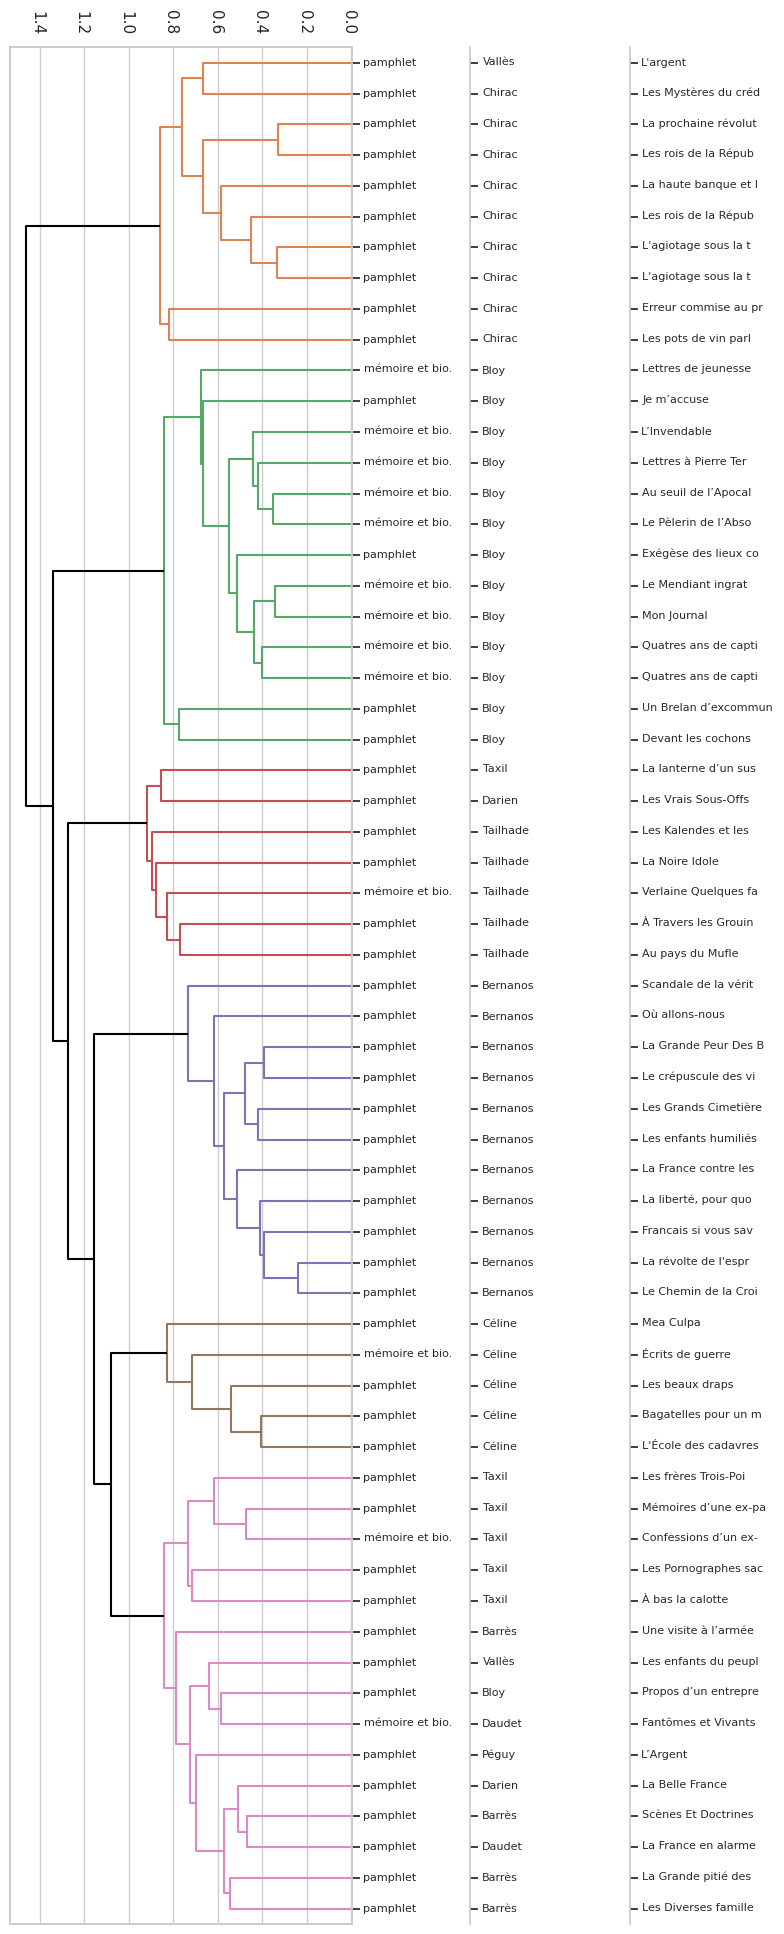
\includegraphics[width=0.60\textwidth]{img/dendogram-corpus-2-PamMem.png }
\caption{Dendrogramme de classification ascendante hiérarchique, Corpus 2, Genres pamphlet-mémoire et biographie, 1 ngram de mot, 12077 / 102851 features, 25 non nulle}
\label{'fig:dendogram-corpus-2-PamMem'}
\end{figure}

\begin{figure}[H]
\centering %
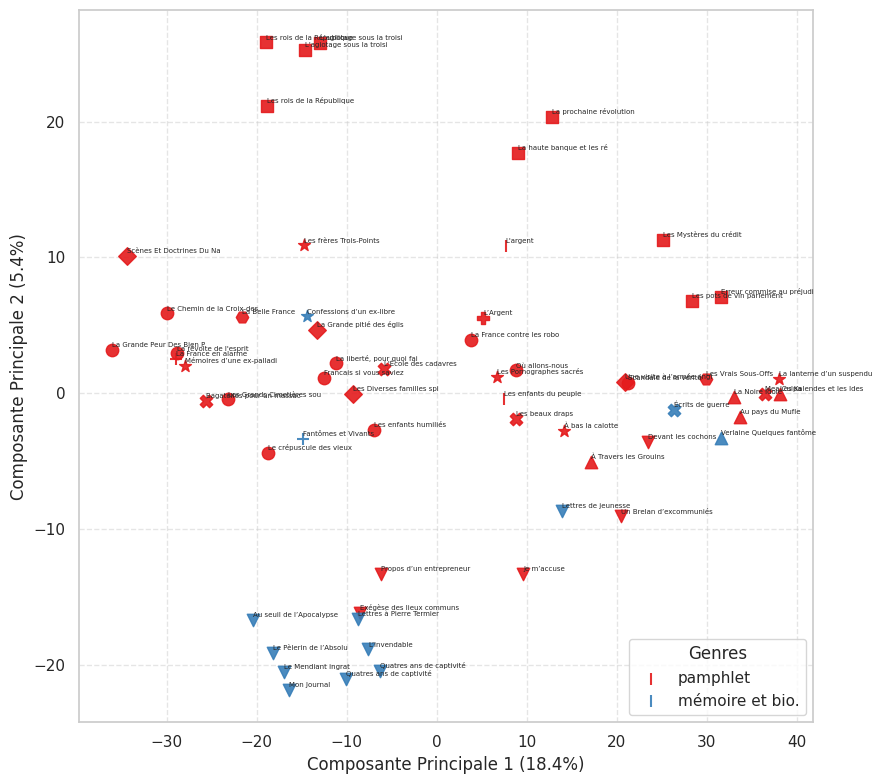
\includegraphics[width=1\textwidth]{img/ACP-corpus-2-PamMem.png}
\caption{Analyse en composantes principales, Corpus 2, Genres pamphlet-mémoire et biographie}
\label{'fig:ACP-corpus-2-PamMem'}
\end{figure}

\begin{figure}[H]
\centering %
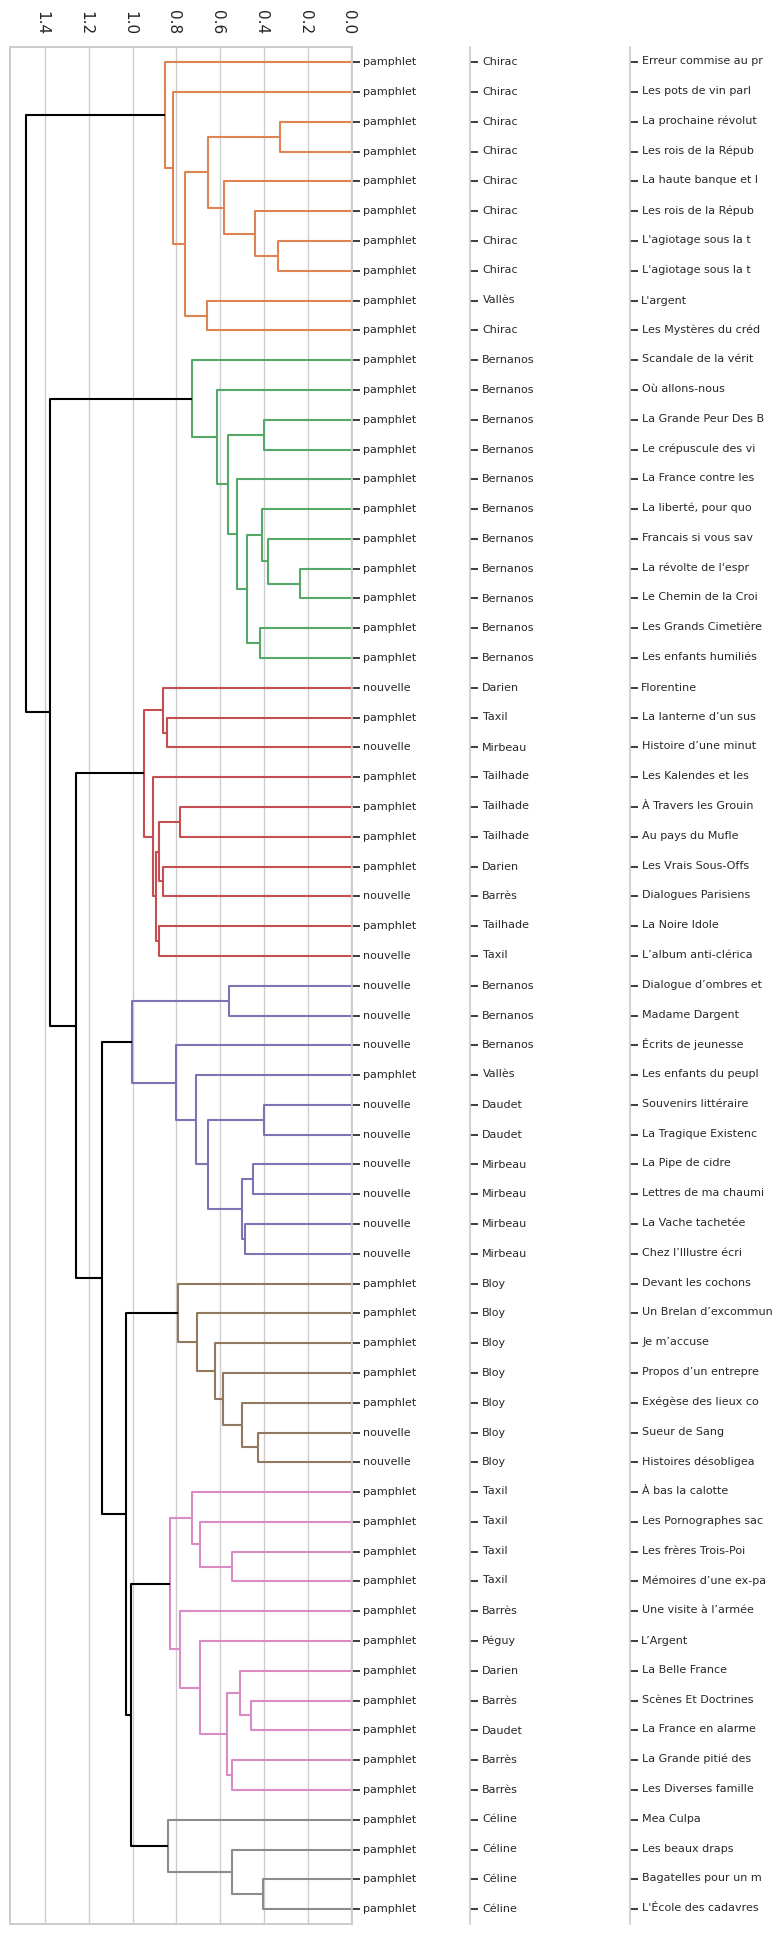
\includegraphics[width=0.60\textwidth]{img/dendogram-corpus-2-PamNouvelle.png}
\caption{Dendrogramme de classification ascendante hiérarchique, Corpus 2, Genres pamphlet-nouvelle, 1 ngram de mot, 11814 / 93079 features, 40 non nulle}
\label{'fig:dendogram-corpus-2-PamNouvelle'}
\end{figure}


\begin{figure}[H]
\centering %
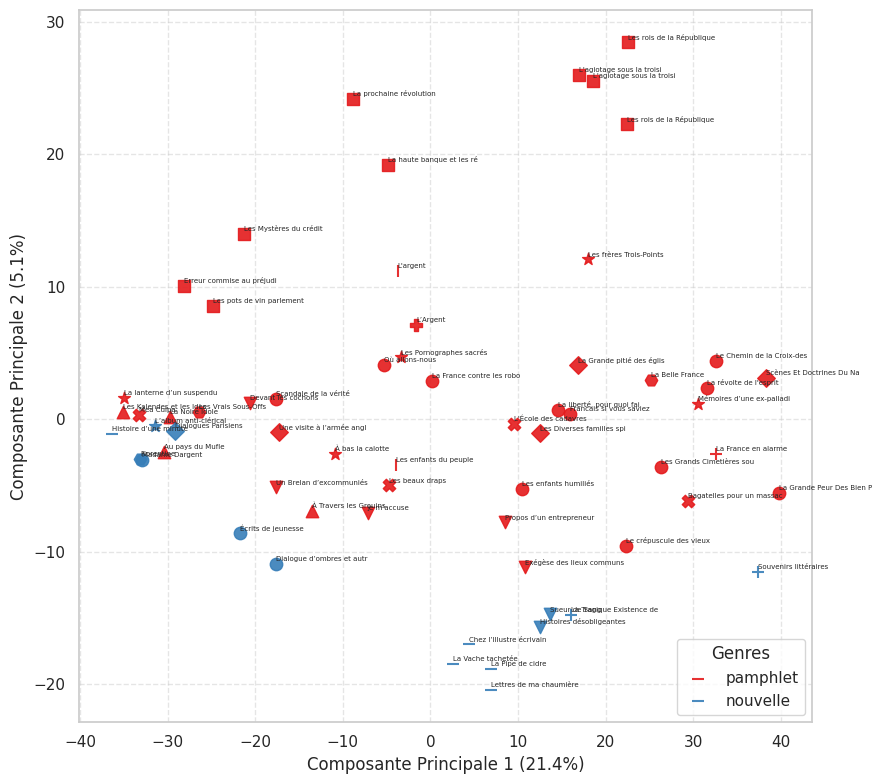
\includegraphics[width=1\textwidth]{img/ACP-corpus-2-PamNouvelle.png}
\caption{Analyse en composantes principales, Corpus 2 Genres pamphlet-nouvelle}
\label{'fig:ACP-corpus-2-PamNouvelle'}
\end{figure}